\section{Implementation}
\label{sec:implementation}

\begin{figure}
\centering
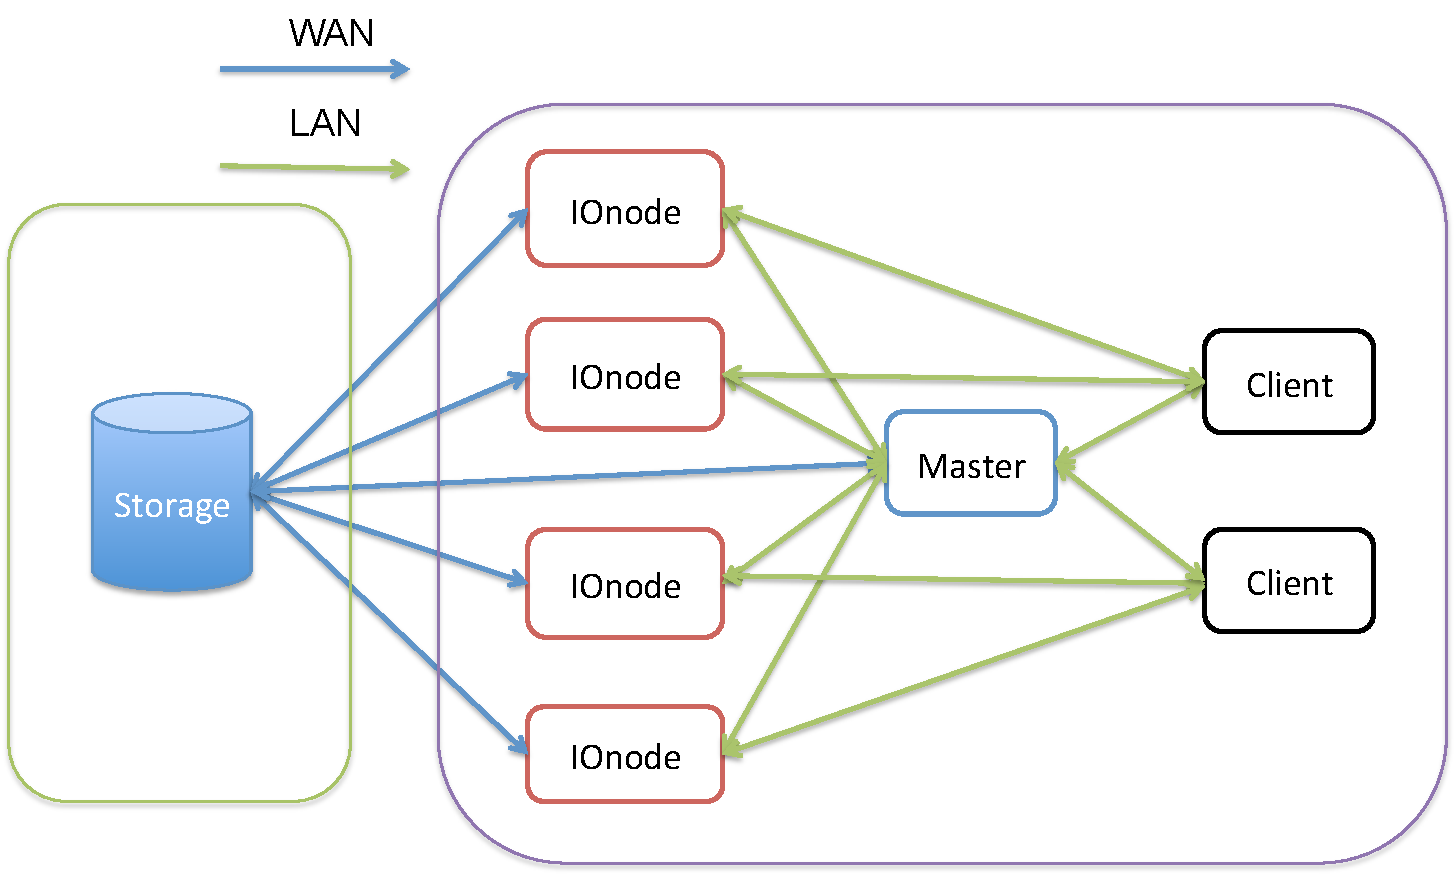
\includegraphics[width=8cm]{img/prototype_overview}
\caption{overview of prototype}
\label{overview of prototype}
\end{figure}

In order to evaluate our architecture in a real environment and compare with current architecture, we implemented a prototype. 
In our architecture there are several global data such as total number of burst buffer nodes,
buffered file information. need to be shared between all nodes.
And since in our proposal architecture, numbers of burst buffer nodes can be dynamically determined,
a global scheduler is needed to decide when and how nodes are added and removed, these decision should be made based on global work load and local work load.
Also a scheduler is needed to handle the operation like re-balance of buffered data when nodes addition, and data write back when nodes deletion.

For above reasons in this implementation, we adopted master-worker model, a master is designed to store global information and interactive with client daemon, as well as serve as a scheduler.
The architecture of our prototype is described as Figure \ref{overview of prototype}

In our architecture, there are three types of nodes:
\begin{itemize}
	\item A master node manages all IOnodes information, maintains a set of buffered file meta data, handles operation like IOnode addition and deletion etc., and interact with clients.
	\item There are several I/O nodes response for actually storing data.
	\item A daemon runs on each client machine serving for communication with
	master and IOnodes, in order to hide architecture detail from user.
\end{itemize}

The shared storage system are mounted on both master and I/O nodes, both of master and I/O nodes have the same assess permission to the shared file system.

\subsection{File Chunk}
In our implementation, files are usually stored in more than one I/O node depends on the files' size and numbers of I/O nodes available.
Files are divided into mutable-size \emph{chunks}, each I/O node store one chunk.
Such one I/O node one chunk design simplified our data layout design, and operations in I/O nodes addition and deletion.
For each chunk we adopted a \emph{dirty flag}, in order to decide whether this chunk has been modified.
In write back phase, only the modified chunk needs to be written back to storage.
This dirty flag can reduce the write back data size and thus reduce the Internet congestion.

Applications usually generate various sizes of files\ref{iosize}, since in our architecture, memory is precious resources, more memory means we can buffer more files,
mutable size chunk design avoid the disadvantage of memory waste in fixed-size chunk design, and enable us just to allocate requested size of memory.
However such one I/O node one chunk design and mutable size has some disadvantages. First master must maintain the chunk size of each file, this put a burden on master.
Second, for a large file the chunk size will become very large, cause a coarse-grained write back control, and reduce the performance gained by dirty flag.
Finally, since the chunk size is decided by file size, and one I/O node store only one chunk, it is difficult to change buffered file size without adding to or removing some I/O nodes from file.

\subsection{Master Node}
In our master-IOnode model, master node is the supervisor of the entire system,
master node is in charge of interactive with client, make file chunk placement, and handle file operations including file open, read and write.
Master node also manage the I/O nodes and schedule events like node registration at node setup phase, addition and deletion.
In order to master node majorly maintain following two data structures:
\begin{itemize}
  \item I/O nodes information: including node ip address, total memory and available memory.
  \item file meta data: including file path, file id, total file size, access control, chunk size, dirty flag and a map from chunks to I/O nodes.
\end{itemize}

Since only master has the global knowledge of file chunk placement, client must connect to master to get these information.
However, in such master-worker model, master is easy to become a bottleneck of the whole system,
thus we have to minimize the master involvement in file operation, client asks master about the file meta data, including the chunk placement information,
then client caches these information and connect to I/O nodes directly for sending or receiving data.

\subsection{File operations}

\begin{figure}
\centering
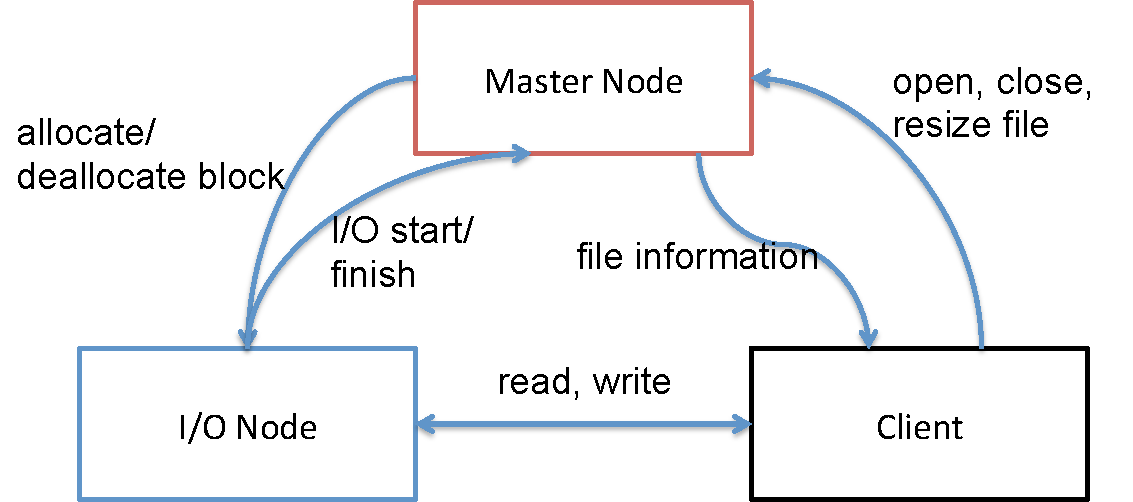
\includegraphics[width=8cm]{img/file_operation}
\caption{Details of File Operation}
\label{implementation:file operation}
\end{figure}

In this section we give more details about the file operation in our implementation, including open, read and write.

When a user try to open a file, client first send file path, access mode to master via client daemon, for unbuffered file, master record the file information , and assign a file id,
and then send the file id to client.

After file opened, client can use file id to send read or write request, in order to monitor the file access and make swap schedule, all the read and write request are first send to master,
after receive the request, for file opened for reading request,
master get the file size from shared storage, and assign several I/O nodes to this file according to file size.
As for file opened in only writing since the file need to be create, master get file size from client daemon and assign I/O nodes
after that master send I/O nodes ip address as well as the map information from chunks to I/O nodes to client daemon, client cache these information.

\subsection{Limitation}
\begin{color}{red}
\begin{itemize}
  \item one I/O node one data chunk reduce the performance gains by using dirty flag.
  \item blocking I/O node
\end{itemize}
\end{color}
